\documentclass[10pt]{article}

\usepackage{url}
\usepackage{graphicx}
\usepackage{times}

\begin{document}

\title{Ibis Communication Library Programmer's Manual}

\author{http://www.cs.vu.nl/ibis}

\maketitle

\section{Introduction}

This manual explains how to program applications using the Ibis
communication library. Ibis is a portable, high performance, Java based
library. For information on how to run applications using this library,
see the Ibis user's manual, available in the Ibis distribution in the
\texttt{doc} directory, or on the Ibis
website\footnote{\url{http://www.cs.vu.nl/ibis}}.

In this manual, we will focus on concepts and methods rather than
details like exact parameters of functions. For this type of
information, see the Javadoc for Ibis. This is available in the
\texttt{javadoc} directory of the distribution, and on the website.

This manual is split up into several different sections. First, we will
explain the different parts of the IPL, the interface to the Ibis
communication library. Second, we explain how to compile applications
which use Ibis. Last, we will give some examples 
to show how to use Ibis in practice.

\section{IPL Overview}

%-- ipl picture, implementations, upcalls, identifiers, instances

\begin{figure} \centering
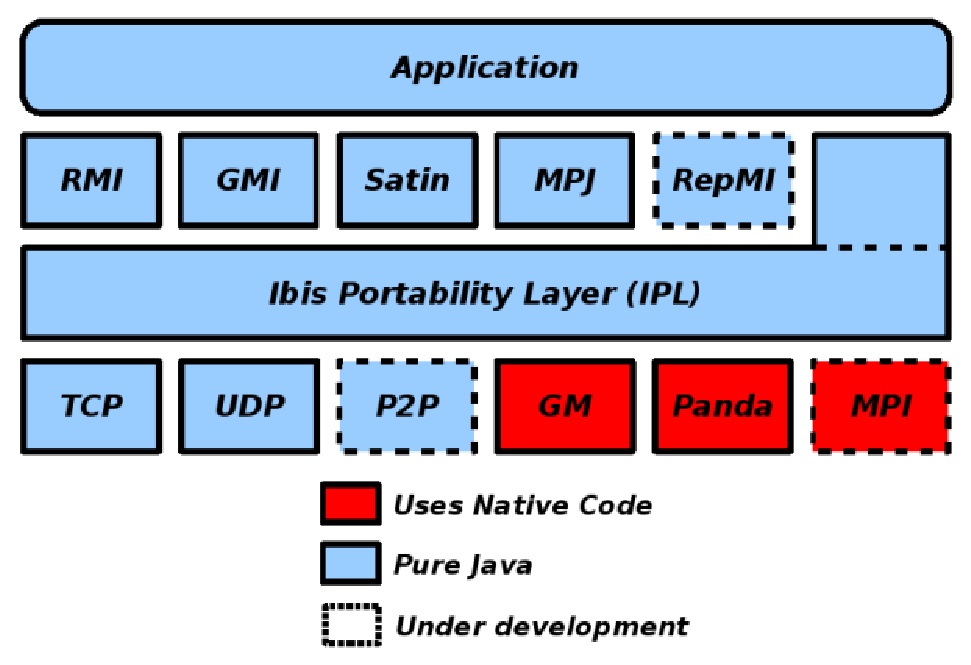
\includegraphics[width=0.9\textwidth]{../images/old-ibis-design.eps}
\caption{Ibis design overview} \label{design}
\end{figure}

This section will give a high level overview of the different parts of
the IPL.  For an overview of the design of Ibis, see
Figure~\ref{design}. The Ibis communication library is build up around
the \emph{Ibis Portability Layer (IPL)}. This layer offers applications a
grid aware communication library, independent of the actual network
used. Ibis can dynamically select a suitable implementation at run-time.
The Ibis communication library ships with several different TCP based
implementation, but implementations based on native platforms such as
MPI and Myrinet are also possible.

Using the IPL, we implemented several different programming models, such
as the divide-and-conquer Satin model, and the Group Based Method
Invocation(GMI) model. A discussion of these models lies outside the
scope of this manual. For more information on the programming models,
see the Ibis website. As an alternative to using a intermediate
programming model, applications can also be written directly on top of
the IPL. The main target audience of this manual are programmers using
the IPL in an application and programming model writers.

A central concept in the IPL is the \emph{Ibis instance}. In general,
one Ibis instance is created on each machine participating in a
particular distributed application. Each of these instances has a unique
\emph{Ibis Identifier}, used throughout the library to denote this
instance.

Another often used concept is the \emph{upcall}. Upcalls can be used
instead of downcalls(explicit receipt, polling) in a number of cases.
These cases include receiving messages, getting notifications of new
connections, and updates on new Ibis instances joining a computation.

\subsection{Send and Receive Ports}

%-- send port, receive port, connections, porttypes

\begin{figure} \centering

\includegraphics[width=0.5\textwidth]{../images/ports.eps}
\caption{Ibis send and receive port configurations} \label{ports}
\end{figure}

The IPL is based on uni-directional connection oriented pipes. In the
model, \emph{send ports} are connected to \emph{receive ports}. See
Figure~\ref{ports} for some examples. Connecting a single send port to a
single receive port leads to a simple one-to-one connection. But, it is
also possible to connect a send port to multiple receive ports for a
one-to-many multicast, or multiple send ports to a single receive port
for many-to-one client server type communication. Even connecting
multiple send ports to multiple receive ports is possible, although this
many-to-many communication model is currently not supported by the
standard TCP based implementation of Ibis.

\begin{figure} \centering
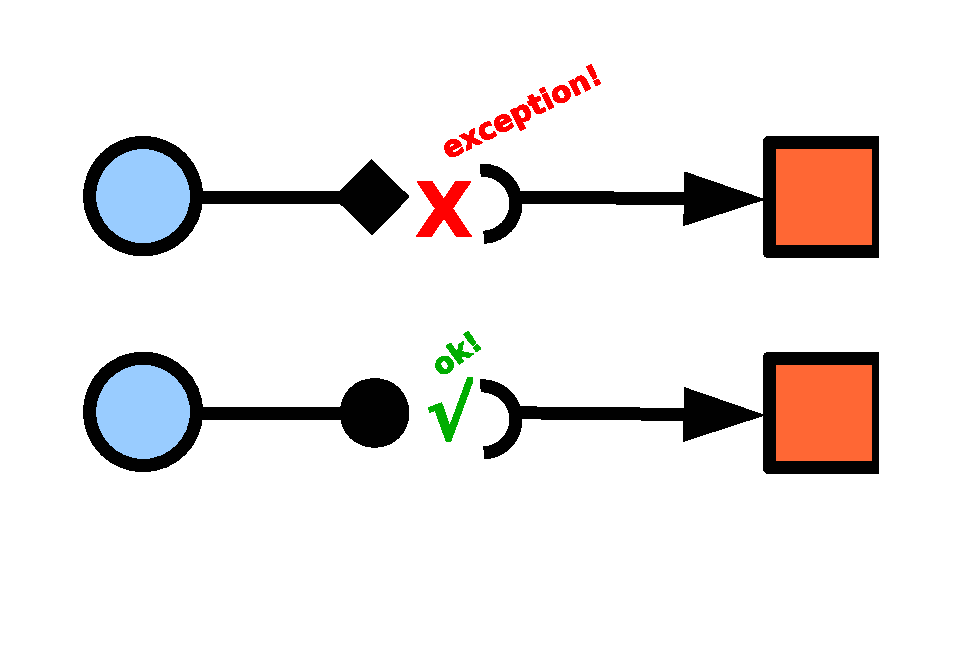
\includegraphics[width=0.5\textwidth]{../images/port_types.eps}
\caption{Port types} \label{port_types}
\end{figure}

Ports in Ibis are typed (see Figure~\ref{port_types}). Types are
determined by the communication pattern (one-to-one, one-to-many,
many-to-one, many-to-many), the type of data that can be send,
reliability, and others. Send ports can only be connected to receive
ports of the same type. This allows for some sanity checks on the
application, and allows Ibis to select the most appropriate
implementation of the communication channel.

\subsection{Messages and Serialization}

%--messages, serialization, bytecode rewriting

Once a connection is established between send and receive ports, data
can now be send. Send and receive ports in Ibis communicate using
messages. A so called \emph{write message} is created at the send port,
and can be filled with all primitive data types of Java such as bytes, integers
and strings, as well as more complex data structures in the form of
Java \texttt{Objects}. Also, arrays of primitive types and object can be
send. When the user is done writing data to a message a \texttt{finish}
message must be called to denote the message has been completed.

Once data is written using a write message at the send port, this
message will arrive at the receive port as a \emph{read message}. There,
the data can be read again using functions equivalent to the ones in
write message. Data must be read from the read message in the same order
as it was written in the write message.

In Ibis, the size of a message is unlimited. However, at any point in
time, only a single message can be active at a port. This allows Ibis to
start sending data to the receiver as soon as it is written in the
message. So, while data is still being written to a message at the
sender, it may already be read at the receiver. This streaming behavior
makes communication in Ibis much more efficient.

Serialization of Objects is the translation of data into bytes suitable for
sending across a network. Ibis is capable of several different versions
of serialization, depending on the needs of the user. These versions
differ in the types of data they support. Some only support sending
bytes, some only primitive types, and some also allow sending objects.

Two different object serialization versions are present in Ibis.  One is
the standard Java object serialization, the other a high-performance
implementation of object serialization. For this high-performance
\emph{Ibis Serialization} implementation to work, an extra step is needed
when compiling the application. Some extra code is generated to
facilitate sending objects efficiently. See Section\ref{compiling} for
more info.

\subsection{Pools and the Registry}

%-- pools, registry, join, leave, died, election, location

Each Ibis instance is a member of a \emph{Pool}. The Ibis
\emph{Registry} keeps track of all the members of the pool, and notifies
all Ibises whenever a new Ibis instance joins this pool, leaves the
pool, or even when a Ibis dies unexpectedly. Applications can use the
registry mechanism to get notified of any changes to the pool.

The Ibis registry also supports \emph{elections}, which can be used to
select Ibis instances which are special such as servers.  Each election
has a unique name in the form of a String, and will elect a winner from
the candidates for this election. Elections are not democratic though,
and usually the first candidate is elected as the winner. It is also
possible to request the outcome of an election without being a
candidate. When the winner of an election leaves the pool, or dies, a
new winner is automatically selected if any new candidate enters the
election.

The registry has a few other features useful for coordinating
distributed computations. One is a \emph{signal} system, where the
registry can send simple string to ibises. This can be used to signal
special events, such as the application terminating. Another feature is
the \emph{sequencer}. The sequencer can be used to get unique sequence
numbers in a distributed fashion. Each call to this function, at
whatever Ibis instance, will yield the next number in the sequence. A
central coordination point is used to implement this reliably.

The normal implementation of the Registry is a central registry service.
This allows for a reliable system, with a good consistency model.
Election are guaranteed to yield the same winner at each Ibis, and any
changes to the membership list of the pool are reported in the same
order at each Ibis. In this model, joins and leaves are guaranteed to be
totally ordered. This implementation does rely on a central server
for coordination. This may lead to inefficiencies, and is also a single
point of failure. So, as an alternative, other, less strict, consistency
models can also be offered.

\subsection{Capabilities}

To facilitate the selection of the best implementation for all the
functionality required of Ibis from a user, Ibis uses a
\emph{capability} based selection mechanism. For each Ibis instance, and
each port type, the user can specify which capabilities are needed. Each
capability enables a certain part of the API. For instance, sending
objects in message is only possible if the "object serialization"
capability is enabled in the port type. Likewise, elections can only be
done if either the "unreliable election" or the "strict election"
capability is enabled. The difference between the two being the
consistency model of the elections. 

\subsubsection{Global Ibis Capabilities}

This is a list of the capabilities for an Ibis. These capabilities
are defined in the \texttt{IbisCapabilities} class of the IPL. See the
Javadoc.  

\begin{description}

\item[SIGNALS]
Enables the signal sending and receiving functionality of the registry.

\item[MEMBERSHIP\_UNRELIABLE] 
Enables the membership information functionality of the registry. The
registry can notify the user whenever a new ibis joins the pool or a
ibis leaves the pool, or dies. This is not reliable though, and some
changes to the pool may not be reported. Also, the order in which
changes are reported is not fixed.

\item[MEMBERSHIP\_TOTALLY\_ORDERED]
As above, but with a better consistency model. Each and every change to
the pool will be reliably reported, and the order of these changes is
fixed for the entire pool. All ibises get the changes in the same,
globally unique, order.

\item[ELECTIONS\_UNRELIABLE]
Enables elections. When doing elections it is possible that some
election results are not available, and if the same election is done at
two different ibises, the result may be different.

\item[ELECTIONS\_STRICT]
Indicates elections are supported, and they adhere to the following 
consistency model: Each election has a single, unique winner at any
given point in time, and all Ibis instances in a pool get all updates
to the election result, and in the same order.

\item[CLOSED\_WORLD]
The Ibises in the pool are determined at the start of the
run. After these Ibises have joined, any further requests to join the
pool will be denied. Requires the number of Ibises in the pool to be
known in advance. This can be set using a property (see
Section~\ref{properties}).

\item[MALLEABLE]
Requests malleability support from Ibis. Some implementations of Ibis
(such as an Ibis based on MPI), may not support Ibises joining the pool
after it has initially been created.

\end{description}

\subsubsection{Port Type Capabilities}

This is a list of capabilities for port types. For each port types,
a single capability for the allowed connection types (one-to-one,
multicast, etc) must be selected, as well as a type of
serialization(bytes only, primitive types, objects, etc). These
capabilities are defined in in the \texttt{PortType} class of the IPL.

\begin{description}
\item[CONNECTION\_ONE\_TO\_ONE]
One-to-one (unicast) communication is supported.

\item[CONNECTION\_ONE\_TO\_MANY]
one-to-many (multicast) communication is supported
(in Ibis terms: a send port
may connect to multiple receive ports).

\item[CONNECTION\_MANY\_TO\_ONE]
many-to-one communication is supported (in Ibis terms: multiple
send ports may connect to a single receive port).

\item[CONNECTION\_MANY\_TO\_MANY]
many-to-one communication is supported (in Ibis terms: multiple
send ports may connect to multiple receive ports).

\item[CONNECTION\_DOWNCALLS]
connection downcalls are supported. This means that the user can
invoke methods to see which connections were lost or created.

\item[CONNECTION\_DOWNCALLS]
connection upcalls are supported. This means that an upcall handler can
be installed that is invoked whenever a new connection arrives or a
connection is lost.

\item[CONNECTION\_TIMEOUT]
Enabled the usage of timeouts in connection attempts.

\item[RECEIVE\_EXPLICIT]
Explicit receive is supported. A message can be received by directly
requesting the reception of a message from the receive port.

\item[RECEIVE\_TIMEOUT]
Explicit receive with a timeout is supported.

\item[RECEIVE\_POOL]
Non-blocking version of explicit receipt is supported.

\item[RECEIVE\_AUTO\_UPCALLS]
Upcalls are supported and polling for them is not required.
This means that when the user creates a receive port with an upcall
handler installed, when a message arrives at that receive port, 
this upcall handler is invoked automatically.

\item[RECEIVE\_POLL\_UPCALLS]
Upcalls are supported but polling for them is required. So, a user must
call the \texttt{poll} function in the receive port to reliably receive
messages, but these messages will be delivered using an upcall.

\item[COMMUNICATION\_FIFO]
Messages from a send port are delivered to the receive ports it is
connected to in the order in which they were sent.

\item[COMMUNICATION\_NUMBERED]
All messages originating from any send port of a specific port type have
a sequence number. This allows the application to do its own sequencing.

\item[COMMUNICATION\_RELIABLE] 
Reliable communication is supported, that is, a reliable communication
protocol is used.  When not specified, an Ibis implementation may be
chosen that does not explicitly support reliable communication.

\item[SERIALIZATION\_BYTE]
Only the methods \texttt{readByte()}, \texttt{writeByte()}, \\
\texttt{readArray(byte[])} and \texttt{writeArray(byte[])} are
supported in read and write messages.

\item[SERIALIZATION\_DATA]
Only \texttt{read()}/\texttt{write()} and
\texttt{readArray()} and \\
 \texttt{writeArray()} of primitive types are
supported in read an write messages.

\item[SERIALIZATION\_OBJECT]
Some sort of object serialization is supported.
This requires user-defined
\texttt{writeObject()}/\texttt{readObject()} methods to be symmetrical,
that is,
each write in \texttt{writeObject()} must have a corresponding read
in \texttt{readObject()} (and vice versa).

\item[SERIALIZATION\_OBJECT\_SUN]
Sun serialization is supported through \\
\texttt{java.io.ObjectOutputStream} and
\texttt{java.io.ObjectInputStream}).

\item[SERIALIZATION\_OBJECT\_IBIS]
Ibis serialization is supported. This is more efficient than sun
serialization, but may have some limitations. For instance, versioning
of objects is not supported.

\end{description}

\subsection{Properties}
\label{properties}

Properties are used in Ibis for setting configuration options at
run-time. These include where to find the Ibis Implementations and the name
of the pool to join. Properties can be passed to a Ibis when it is
created, but Ibis can also add properties specified on the command line
by default. See the user's guide for more information on the various
properties of Ibis and their usage.

\section{Compiling applications}
\label{compiling}

%-- add ipl.jar to classpath, rewrite using ibisc, example ant build file.

Applications that use Ibis can be compiled as any normal Java
application. The \texttt{ipl.jar} needs to be added to the
classpath when compiling (and running) an Ibis application. For the
serialization of Ibis to function correctly, one additional step is
required after compiling: the code for writing and reading objects must
be generated. A Ibis compiler application is available for
this purpose. It can be run by using the \texttt{ibisc}
script in the \texttt{bin} directory of the distribution. The ibis
compiler needs to be passed the class files of the application, either
as a directory containing classes, or as a jar file.

Ibisc can also be called from \texttt{ant}, the make-like build system
for Java\footnote{\url{http://ant.apache.org}}. An example of a build
file which calls the ibis compiler is available in the \texttt{examples}
directory of the distribution. The relevant piece of script is this:

\begin{quote}
\begin{verbatim}
<java classname="ibis.compile.Ibisc"
      taskname="Ibisc"
      failonerror="true"
      fork="true">
          <arg line="ipl-examples2.0rc2.jar" />
          <classpath refid="default.classpath" />
</java>
\end{verbatim}
\end{quote}

It runs the ibis compiler on the jar file that has just been created
from the compiled classes. It sets the classpath to the same classpath
used to compile the application.

\section{Tutorial}

%-- include tutorial.tex
\input tutorial

\section{Further Reading}

The Javadoc included in the \texttt{javadoc} directory has detailed
information on all classes and their functions.

The Ibis web page \url{http://www.cs.vu.nl/ibis} lists all
the documentation and software available for Ibis, including papers, and
slides of presentations.

For detailed information on running an Ibis application see the
User's Manual, available in the docs directory of the Ibis
distribution.

\end{document}
